A top down approach was applied for identifying the major components in the system. Client's requirements were the starting point for identifying those components. They were
clear and simple enough to create a high level view of the framework , with which to explain the framework's basic behaviour and how it's going to work see figure ~\ref{fig:sprints}. 

\begin{figure}[htp]
\centering
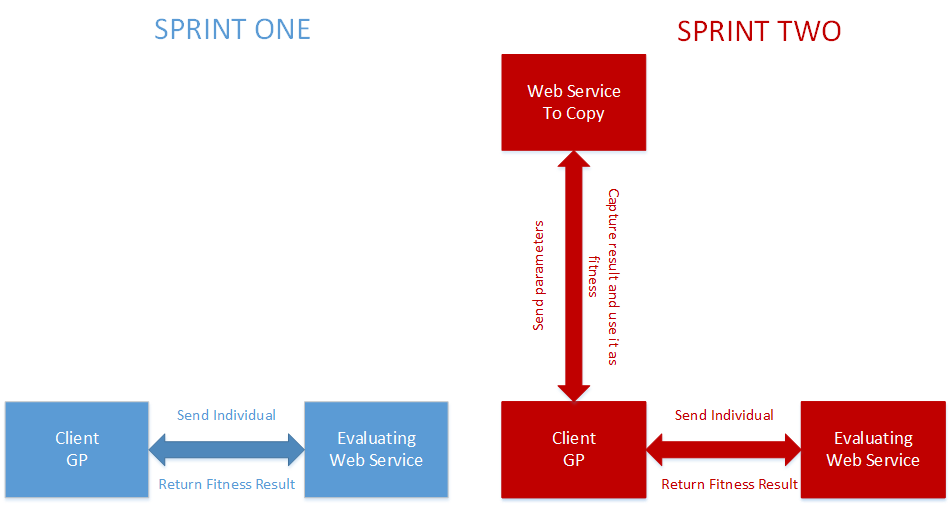
\includegraphics[scale=0.7]{Figures/sprints.png}
\caption{Top level view of sprint one and two}
\label{fig:sprints}
\end{figure}

By displaying the way the high level components communicate it was later possible to identify lower level ones.
